\documentclass[12pt,fleqn]{article}
\usepackage{../lecture-notes/vkCourseML}
\usepackage{lipsum}
\usepackage{indentfirst}
\usepackage{graphicx}
\usepackage{animate}
\usepackage{hyperref}
\graphicspath{{./figures/}}
\title{Машинное обучение, ФКН ВШЭ\\Семинар №25\\Отбор признаков}
\author{}
\date{}

\begin{document}
	\maketitle
	
	Зачастую бывает, что данные обладают множеством признаков, и далеко не все из них могут быть полезны в задачах машинного обучения: вполне возможно, что какие-то из них имеют слабое влияние на результат работы модели или не имеют влияния вообще, являясь скорее шумом, а не чем-то полезным. Так как включение таких признаков в процесс обучения замедляет и усложняет его, в этом семинаре мы обсудим методы, позволяющие отобрать среди признаков наиболее важные, уменьшая время и память, необходимые для работы алгоритма, жертвуя при этом незначительным (в идеале – никаким) изменением качества модели.
	
	\section{Корреляция}
	
	Один из вариантов измерения важности признаков -- их коррелированность с целевой переменной. Как мы помним, для двух случайных величин $ X $ и $ Y $, распределение которых известно, коэффициент корреляции рассчитывается по формуле:

	\[
	corr(X, Y) =
	\dfrac{cov(X, Y)}{\sqrt{\mathbb{D}[X]\mathbb{D}[Y]}} =
	\dfrac{\mathbb{E}\left[\left(X - \mathbb{E}[X]\right)\left(Y - \mathbb{E}[Y]\right)\right]}{\sqrt{\mathbb{D}[X]\mathbb{D}[Y]}}.
	\]

	Коэффициент принимает значения от $ -1 $ до $ 1 $ и показывает уровень влияния случайных величин друг на друга. Чем меньше абсолютное (это важно!) значение коэффициента корреляции, тем менее важными можно считать переменные в задаче предсказания значения одной из них с помощью другой. Тогда мы можем отбросить признаки с наименьшим коэффициентом корреляции (например, отсечь по некоторому значению или отбросить выбранную долю наименее коррелированных с целевой переменной признаков) и обучаться на уже усечённой выборке данных, экономя память и время.

	Однако в машинном обучении мы обычно работаем не с известными случайными величинами, а с выборками данных, про распределение которых мы ничего не знаем. Тут на помощь приходят несколько способов расчёта корреляции:

	\newpage

	\subsection{Коэффициент корреляции Пирсона}

	Данный метод просто заменяет все величины на их выборочные аналоги, переходя от вероятностных распределений к наблюдаемым данным:

	\[
	r(X, Y) =
	\dfrac{\sum_{i = 1}^{\ell}\left(\left(X_{i} - \overline{X}\right)\left(Y_{i} - \overline{Y}\right)\right)}{\sqrt{\left(\sum_{i = 1}^{\ell}\left(X_{i} - \overline{X}\right)^{2}\right)\left(\sum_{i = 1}^{\ell}\left(Y_{i} - \overline{Y}\right)^{2}\right)}}.
	\]

	Если в задаче линейной регрессии отсутствует регуляризация, то оптимальный вес признака $ x_{i} $ будет равен $ w_{i} = \dfrac{\sigma(y)r(x_{i}, y)}{\sigma(x_{i})} $, где $ \sigma(\cdot) $ обозначает среднеквадратичное отклонение.

	\subsection{Коэффициент ранговой корреляции Кендалла}

	Идея этого способа подсчёта корреляции в том, чтобы посмотреть на согласованность порядков величин $ X $ и $ Y $. Назовём пару $ (i, j) $ согласованной, если верно $ \sign(X_{i} - X_{j}) = \sign(Y_{i} - Y_{j}) $. Тогда, если согласованных пар $ S $, а несогласованных – $ R $, то коэффициент ранговой корреляции Кендалла может быть посчитан как:

	\[
	\tau(X, Y) =
	\dfrac{S - R}{S + R} =
	\dfrac{2(S - R)}{\ell(\ell - 1)} =
	\dfrac{2}{\ell(\ell - 1)}\left(\left(\dfrac{\ell(\ell - 1)}{2} - R\right) - R\right) = 1 - \dfrac{4R}{\ell(\ell - 1)}.
	\]

	Если мы хотим убрать $ S $, это можно сделать с помощью индикаторов:

	\[
	\tau(X, Y) =
	1 - \dfrac{4R}{\ell(\ell - 1)} =
	1 - \dfrac{4\sum_{i = 1}^{\ell - 1}\sum_{j = i + 1}^{\ell}[\sign(X_{i} - X_{j}) \neq \sign(Y_{i} - Y_{j})]}{\ell(\ell - 1)}.
	\]

	Таким образом, данный коэффициент корреляции является мерой упорядоченности последовательностей относительно друг друга.

	\subsection{Коэффициент ранговой корреляции Спирмена}

	В данном методе также важен относительный порядок внутри выборки. Обозначим $ R_{i} = j : X_{(j)} = X_{i} $, $ S_{i} = j : Y_{(j)} = Y_{i} $ (другими словами, данные величины показывают, какое место занимали бы рассматриваемые переменные в упорядоченной выборке), $ d_{i} = R_{i} - S_{i} $. Тогда коэффициент корреляции Спирмена вычисляется следующим образом:

	\[
	\rho(X, Y) =
	1 - \dfrac{6\sum_{i = 1}^{\ell}d_{i}^{2}}{\ell(\ell^{2} - 1)} =
	1 - \dfrac{6\sum_{i = 1}^{\ell}\left(R_{i} - S_{i}\right)^{2}}{\ell(\ell^{2} - 1)}.
	\]

	Обычно верно $ |\rho(X, Y)| \geqslant |\tau(X, Y)| $. Как видим, ни этот, ни предыдущий метод подсчёта коэффициента корреляции не использует никакой информации о данных, кроме некоторого их упорядочивания (ранжирования). Если некоторые объекты имеют одинаковое значение (ранг), описанные коэффициенты несколько изменяются.

	\subsection{Коэффициент корреляции знаков Фехнера}

	Данный способ подсчёта коэффициента корреляции, пожалуй, является самым простым с точки зрения вычисления и самой идеи: назовём пару $ (X_{i}, Y_{i}) $ согласованной, если верно $ \sign(X_{i} - \overline{X}) = \sign(Y_{i} - \overline{Y}) $. Если согласованных пар $ C $, а несогласованных – $ H $, то коэффициент корреляции знаков Фехнера будет равен:

	\[
	i(X, Y) = \dfrac{C - H}{C + H} = \dfrac{(\ell - H) - H}{\ell} = 1 - \dfrac{2H}{\ell} = 1 - \dfrac{2\sum_{i = 1}^{\ell}[\sign(X_{i} - \overline{X}) \neq \sign(Y_{i} - \overline{Y})]}{\ell}.
	\]

	Данный коэффициент корреляции можно считать более грубой и простой версии коэффициента корреляции Пирсона, впрочем, иногда он тоже может быть вполне полезен.

	\subsection{Вычислительная сложность}

	Давайте посмотрим на формулы и поймём, какую вычислительную сложность имеют описанные выше способы подсчёта коэффициента корреляции:

	\begin{enumerate}
		\item Коэффициент корреляции Пирсона – требует подсчёта средних и различных разностей с ними, сложность $ O(\ell) $.
		\item Коэффициент ранговой корреляции Кендалла – требует подсчёта некоторых значений для каждой пары объектов, сложность $ O(\ell^{2}) $.
		\item Коэффициент ранговой корреляции Спирмена – требует сортировки и линейного числа подсчётов, сложность $ O(\ell\log(\ell)) $.
		\item Коэффициент корреляции знаков Фехнера – требует подсчёта средних и различных выражений с ними, сложность $ O(\ell) $ (но быстрее метода Пирсона).
	\end{enumerate}

	Конечно, относительно самого процесса обучения ресурсы, затрачиваемые на подсчёт корреляций, довольно малы, но с ростом размера данных и они начинают иметь весомое значение, так что важно помнить асимптотику описанных выше алгоритмов.



	\subsection{Плюсы и минусы}

	Конечно, отбор признаков в принципе и по коэффициенту корреляции в частности обладает рядом преимуществ, но присутствует и ряд важных проблем:
	\begin{itemize}
		\item[$ + $] Отбор признаков позволяет снизить время и объём памяти, необходимые для работы модели.
		\item[$ - $] Скорее всего, произойдёт некоторая потеря качества.
		\item[$ + $] Коэффициент корреляции умеет хорошо <<замечать>> линейные (в случае с ранговой корреляцией – любые монотонные) зависимости между переменными, в этом случае он хорошо подходит для отбора признаков.
		\item[$ - $] Любые нелинейные и/или немонотонные зависимости становятся проблемой при отборе по коэффициенту корреляции. Если посчитать коэффициент корреляции для периодической или чётной относительно какой-то точки зависимости, он выйдет близким к нулю, и подобный признак будет отсеян, хотя мог бы быть очень ценен если не сам по себе, то после некоторого преобразования. Для лучшей демонстрации можно взглянуть на рис.~\ref{fig:corr}:
		\begin{center}
			\begin{figure}[!htb]
				\centering
				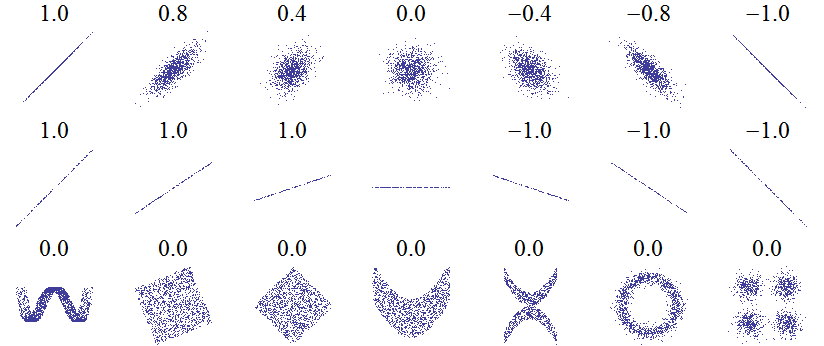
\includegraphics[width = 0.9\linewidth]{Correlation_examples.png}
				\caption{Распределения $ (x, y) $ с соответствующими коэффициентами корреляций}\label{fig:corr}
			\end{figure}
		\end{center}
		Как можно увидеть, коэффициент корреляции отражает <<зашумлённость>> линейной зависимости (верхняя строка) (это как раз то, что нужно и где коэффициент корреляции хорошо справляется со своей задачей), но не описывает наклон линейной зависимости (средняя строка) (что, впрочем, не проблема, как раз коэффициенты у линейной зависимости подобрать можно), и совсем не подходит для описания сложных, нелинейных зависимостей (нижняя строка) (такие зависимости коэффициент корреляции просто не обнаруживает и бракует); для распределения, показанного в центре рисунка, коэффициент корреляции не определен, так как дисперсия $ y $ равна нулю. Если мы хотим, чтобы отбор признаков по коэффициенту корреляции не пропускал более сложные зависимости, придётся сгенерировать новые признаки, являющиеся преобразованиями над исходными, и искать наиболее коррелированные ещё и среди них. Тут сразу видна проблема: мы хотели избавиться от признаков, а в такой ситуации нам придётся генерировать ещё больше. К тому же, нет гарантий, что у нас получится найти удачную комбинацию старых признаков, имеющую сильную корреляцию с целевой переменной.
		
		Коэффициенты ранговой корреляции позволяют обнаруживать монотонные зависимости, но ничего не говорят об их виде: зависимость может быть логарифмической, полиномиальной, экспоненциональной или любой другой (например, $ y = 2x + \sin(x) $ тоже получила бы высокий коэффициент корреляции, но восстановление исходной зависимости от этого сильно легче бы не стало).
	\end{itemize}

	Что ж, теперь давайте поговорим про другие методы отбора признаков.

	\section{Другие методы отбора признаков}

	Мы разберём два других метода отбора признаков, которые напоминают процессы, происходящие в реальном мире и изучаемые физикой и биологией соответственно. Начнём мы с <<физического>> алгоритма.

	\subsection{Алгоритм имитации отжига}

	Идея этого алгоритма в следующем: изначально мы начинаем со случайного подмножества признаков (размер подмножества будет зафиксирован на протяжении всего алгоритма), находясь в <<разогретой>> среде. Для данного набора признаков мы считаем качество модели, после чего случайным образом выбираем некоторое другое подмножество признаков, для которого также считаем качество. Если оно оказалось выше, мы перемещаемся в новую точку. Иначе мы либо остаемся, либо перемещаемся с некоторой вероятностью, положительно зависящей от температуры и отрицательно -- от разницы в метрике качества. Повторяем описанный процесс до тех пор, пока температура не упадёт до нуля, обозначая <<замерзание>> системы и остановку на текущем подмножестве признаков.

	Обсудим плюсы и минусы данного алгоритма относительно рассмотренных выше вариантов отбора признаков:
	\begin{itemize}
		\item[$ + $] Правила изменения температуры и вероятности перемещения можно настраивать, изменяя результат работы алгоритма.
		\item[$ - $] Алгоритм недетерминированный и может показывать неожиданно плохие результаты (застрять в локальном максимуме, начать с неудачного подмножества). Неверная настройка процесса падения температуры и правил перемещения также может навредить, препятствуя получению хорошего результата.
		\item[$ + $] Так как алгоритм не бездумно отбирает самые коррелированные признаки, может быть обнаружена комбинация, дающая хорошее качество, даже если по отдельности признаки несут мало информации.
		\item[$ - $] На каждом шаге нужно обучать новую модель, что очень затратно по времени. Такой алгоритм работает гораздо медленнее сортировки по коэффициенту корреляции.
	\end{itemize}

	Подводя итог: данный алгоритм обладает своими плюсами и минусами, частично совпадающими с проблемами отбора признаков по коэффициентам корреляции. Он может работать как хуже, так и лучше рассмотренных ранее методов. В случае, когда важно получить как можно более высокое качество при большом запасе времени, данный алгоритм точно стоит включить в рассмотрение, возможно, дав ему несколько попыток и меняя правила падения температуры. В таких условиях алгоритм отжига может показать отличные результаты, что особенно ценно, если постоянно появляются новые данные, и важно показывать на них как можно более высокое качество.

	\subsection{Генетический алгоритм}

	Данный алгоритм симулирует процесс естественного отбора и имеет несколько основных этапов, которые будут описаны ниже. Также, как и в случае с алгоритмом имитации отжига, размер подмножества признаков фиксируется заранее и не меняется в процессе работы алгоритма.

	\paragraph*{Создание начальной популяции.} Случайным образом генерируются особи (каждая особь характеризуется своим подмножеством признаков), каждый признак должен появляться хотя бы в одной (больше появлений, конечно, даст большее качество) особи. Для каждой особи вычисляется качество модели на её подмножестве признаков (стоит заметить, что даже если начальная популяция с точки зрения качества получилась не очень удачной, генетический алгоритм с большой вероятностью сможет достаточно быстро улучшить её до приемлемых значений качества). После начинается цикл, повторяющийся до выполнения условия остановки.

	\paragraph*{Скрещивание и мутация.} Данные шаги отвечают за изменение популяции и добавление в неё новых особей. Они могут применяться в любом порядке (или один из них может не применяться вообще), но хотя бы один из двух шагов должен быть выполнен на каждой итерации цикла.

	\subparagraph*{Скрещивание.} Из популяции выбираются родители (обычно берутся два родителя для создания одной новой особи, но можно и больше). Выбирать родителей и скрещивать их можно по-разному. Начнём с процесса выбора родителей:
	\begin{itemize}
		\item Можно выбирать пару родителей случайно (равновероятно или пропорционально качествам особей (или некоторого преобразования над качествами особей)) (панмиксия).
		\item Можно выбрать одного родителя случайно, а второго взять максимально похожим на первого (инбридинг).
		\item Можно выбрать одного родителя случайно, а второго взять минимально похожим на первого (аутбридинг).
	\end{itemize}

	Заметим, что для последних двух вариантов похожесть особей можно измерять по качеству или долее совпадающих признаков (или какого-то более сложного алгоритма, учитывающего, например, частоту появления признаков среди всех особей).

	После выбора семей (групп родителей) следует скрещивание. Здесь идеи во многом похожи на процесс выбора родителей: можно всегда брать признак, если он есть у всех родителей, а остальные брать случайно (например, равновероятно, пропорционально доле родителей, обладающих этим признаком, пропорционально той же доле и качеству родителей или каким-то преобразованием над описанными вариантами), можно все признаки выбирать случайно, можно каким-то образом комбинировать эти методы.

	После всех описанных манипуляций новые особи добавляются в популяцию. Также возможен второй вариант, который может не применяться, дополнять или заменять скрещивание.

	\subparagraph*{Мутация.} На данном шаге мы выбираем особи (как всегда, равновероятно или случайно с определёнными нами вероятностями) и подвергаем их мутации. В данном случае мутация заключается в изменениях выбранных особей, то есть в удалении и добавлении признаков в подмножество признаков данной особи. Делать это можно различными способами, например, равновероятно или используя частоту появления этого признака у других особей. Новые особи добавляются в популяцию, обычно не заменяя старых.

	\paragraph*{Подсчёт качества.} Для каждой новой особи (полученной скрещиванием или мутацией старых особей) обучается модель и подсчитывается качество. Это будет нужно для следующего шага.

	\paragraph*{Отбор.} На данном этапе среди особей проводится отбор, цель которого -- убрать наименее удачные особи и улучшить среднее качество среди популяции в надежде постепенно эволюционировать до оптимальной особи. Отбор опирается на качество особей и может проходить различными способами, например:
	\begin{itemize}
		\item Просто выбрать самые удачные особи, отсеяв остальных.
		\item Устроить <<турнир>>: сталкивать случайно выбранные особи, каждый раз оставляя ту, у которой выше качество, пока не отсеется достаточно.
		\item Отсеивать особ случайно, установив вероятности выживания, пропорциональные качествам особей или преобразованиям над ними.
	\end{itemize}

	Способов проводить отбор заметно больше, это лишь самые некоторые из них. Комбинации разных способов отсеивания также могут быть работоспособными (например, можно каждый раз объявлять несколько самых удачных особей текущего <<неприкосновенными>> и всегда переносить на следующий шаг цикла, а остальных отбирать с помощью <<турнира>>).

	Обычно после этого шага популяция имеет тот же размер, что и до скрещивания и мутации, то есть поддерживается постоянный размер популяции. Однако при желании можно отсеивать как больше особей (в надежде быстрее сойтись к оптимальной особи или просто сократить время работы алгоритма; чем-то схоже с алгоритмом имитации обжига), так и меньше (чтобы алгоритм не сходился слишком быстро при появления некоторого доминирующего вида особей, а также в надежде на то, что мутация или скрещивание не самых удачных особей могут дать хороший результат). В любом случае, после этого шага проверяется условие остановки цикла.

	\paragraph*{Условие остановки цикла.} Есть несколько стандартных условий, выполнение которых останавливает работу генетического алгоритма. Можно использовать для остановки некоторое их подмножество, выполнение хотя бы одного из условий или всех сразу. Классическими условиями остановки являются:
	\begin{itemize}
		\item Прошло некоторое количество времени.
		\item Произошло некоторое количество итераций алгоритма.
		\item Некоторое количество итераций не наблюдается прирост.
		\item Популяция стала достаточно однородной (например, разница в качестве между лучшей и худшей особью упала ниже определённого порога).
		\item Число особей упало ниже какого-то порога (если на каждом шаге цикла отсеивается больше особей, чем добавляется).
	\end{itemize}

	Если какое-то условие или определённый набор условий выполнились, алгоритм завершает свою работу, предъявляя самую удачную особь в качестве результата. Иначе цикл начинается заново.

	Обсудим плюсы и минусы этого алгоритма относительно предыдущих:
	\begin{itemize}
		\item[$ + $] Генетический алгоритм имеет, пожалуй, наибольшие шансы найти оптимальное или близкое к нему с точки зрения качества подмножество признаков, так как проверяет гораздо больше вариантов по сравнению с отбором по коэффициенту корреляции (там вообще проверяется всего один вариант) или алгоритмом имитации отжига (в нём проверяется больше вариантов, но всё ещё куда меньше, чем в генетическом алгоритме). Хоть алгоритм и недетерменированный (можно сделать детерменированную версию, но это теряет большую часть смысла и симуляции естественного отбора), он с большой вероятностью преодолевает локальные максимумы и движется в сторону оптимального подмножества признаков.
		\item[$ - $] За это приходится платить временем работы и памятью: алгоритм хранит всю текущую популяцию (это занимает $ O(sd) $ памяти, где $ s $ -- число особей в популяции, а $ d $ -- размер подмножетсва признаков у одной особи; также есть массив качеств особей, имеющий размер $ O(s) $ и потому не влияющий на асимптотику), а также обучает модель для каждой особи, что гораздо больше, чем количество обучений в алгоритме имитации отжига или тем более при отборе признаков по коэффициенту корреляции.
	\end{itemize}

	В остальном плюсы и минусы схожи с алгоритмом имитации отжига: генетический алгоритм позволяет с большими затратами времени и памяти подобрать наилучший или близкий к нему набор признаков для обучения. С другой стороны, за время его работы можно было бы сгенерировать множество новых признаков, комбинируя старые, и обучить на них алгоритм имитации отжига или провести отбор по коэффициенту корреляции. Генетический алгоритм может как проиграть, так и выиграть таким альтернативам использования ресурсов. Тем не менее, он точно остаётся легитимным (хотя и необычным) способом отбора признаков.

	\subsection{Последнее преимущество над отбором по корреляции}

	Этот момент настолько важен, что вынесен в отдельный пункт. Кроме всех описанных выше проблем, имеющихся у отбора признаков по коэффициентам корреляции, есть ещё один: все переменные должны быть численными. В случае, если одна из двух рассматриваемых переменных или даже обе бинарны, есть некоторые специальные способы подсчёта коэффициента корреляции между ними (коэффициенты корреляции дихотомических переменных). Если же переменная является категориальной, без предварительной обработки и перевода её в численный вид посчитать коэффициент корреляции не представляется возможным. Алгоритм отжига и генетический алгоритм не всегда сталкиваются с такой проблемой (например, когда мы решаем задачу многоклассовой классификации, отбирать признаки с помощью этих алгоритмов можно, а вот посчитать непосредственно корреляцию с целевой переменной -- нет; придётся изобретать велосипеды с численным кодированием). Об этом также следует помнить, когда мы хотим отбирать признаки и думаем, какой метод стоит выбрать.

\end{document}